\documentclass[11pt,a4paper]{article}
\usepackage{iftex}
\ifPDFTeX
  \usepackage[T1]{fontenc}
  \usepackage[utf8]{inputenc}
  \usepackage[magyar]{babel}
  \usepackage{lmodern}
\else
  \usepackage{fontspec}
  \usepackage{babel}
  \babelprovide[main,import]{hungarian}
\fi
\usepackage[a4paper,margin=22mm]{geometry}
\usepackage{microtype}
\usepackage{array,booktabs,tabularx}
\usepackage{enumitem}
\usepackage{tikz}
\usetikzlibrary{positioning,fit,shapes.geometric,arrows.meta}
\usepackage{hyperref}
\hypersetup{colorlinks=true,linkcolor=blue!45!black,urlcolor=blue!45!black,
  pdftitle={Hexagonális területfoglaló játék -- követelményspecifikáció},
  pdfauthor={Szoftverarchitektúrák házi feladat csapata}}
\setlength{\parindent}{0pt}
\setlength{\parskip}{4pt}
\setlength{\emergencystretch}{2em}
\setlist{nosep,leftmargin=*}
\renewcommand{\arraystretch}{1.15}
\clubpenalty=10000
\widowpenalty=10000
\newcolumntype{Y}{>{\raggedright\arraybackslash}X}
% Beadás előtt kitöltendő csapatadatok.
\newcommand{\csapatnev}{Kitöltendő}
\newcommand{\konzulens}{Kitöltendő}
\newcommand{\tagA}{Kitöltendő}
\newcommand{\tagB}{Kitöltendő}
\newcommand{\tagC}{Kitöltendő}
\newcommand{\tagD}{Kitöltendő}
\newcommand{\neptunA}{Kitöltendő}
\newcommand{\neptunB}{Kitöltendő}
\newcommand{\neptunC}{Kitöltendő}
\newcommand{\neptunD}{Kitöltendő}
\newcommand{\emailA}{Kitöltendő}
\newcommand{\emailB}{Kitöltendő}
\newcommand{\emailC}{Kitöltendő}
\newcommand{\emailD}{Kitöltendő}

\begin{document}
\begin{center}
{\Large\bfseries Hexagonális területfoglaló játék\par}
{\large Követelményspecifikáció\par}
BME -- Szoftverarchitektúrák, MSc házi feladat
\end{center}
\textbf{Verzió:} 0.2 -- egyeztetési változat \hfill
\textbf{Dátum:} 2026. október 7.\par
\textbf{Csapat:} \csapatnev \hfill \textbf{Konzulens:} \konzulens

\begin{tabularx}{\linewidth}{@{}YYY@{}}
\toprule
Csapattag neve & Neptun-kód & E-mail-cím \\
\midrule
\tagA & \neptunA & \emailA \\
\tagB & \neptunB & \emailB \\
\tagC & \neptunC & \emailC \\
\tagD & \neptunD & \emailD \\
\bottomrule
\end{tabularx}

\section{Feladatleírás és cél}
Az alkalmazás körökre osztott területfoglaló játék hexagonális rácson.
A játékosok a saját területük színét változtatva terjeszkednek; a játszma
végén a legtöbb mezőt birtokló játékos nyer. Több ember egy számítógépen,
felváltva játszhat, illetve gépi ellenfelek is részt vehetnek.
A játszma helyben menthető, és a böngésző bezárása után is folytatható.

\section{Részletes működés és fő funkciók}
\textbf{F01 -- Új játszma beállítása.}
2--4 résztvevő állítható be, mindegyik emberi vagy gépi játékos; legalább
egy ember szükséges. A résztvevőket sorszám azonosítja. A pálya rögzített,
12~$\times$~10 mezős, hat színnel véletlenszerűen színezett hexrács,
összekötött szemközti szélek nélkül. A kezdőpontok a pálya különböző
sarkain vannak, két játékosnál szemközt. A kezdőszínek különbözők;
a kezdőmezővel összefüggő, azonos színű mezők induláskor már a játékoshoz
tartoznak. A sorrend a résztvevőlista sorrendje.

\textbf{F02 -- Színválasztás és területfoglalás.}
Az aktuális játékos a saját és az ellenfelek jelenlegi színétől eltérő
színt választ. Teljes területe az új színt kapja, majd hozzáolvad minden
új színű, semleges mező, amely ilyen mezők élmenti láncán keresztül
elérhető a területéből. A terjedés a teljes elérhető komponensre kiterjed.
Más játékos mezője nem foglalható el és nem járható át. A nulla új mezőt
adó színváltás is érvényes; ez önmagában nem zárja le a játszmát.

\textbf{F03 -- Körök vezérlése.}
A teljes foglalás után a következő résztvevő lép; az utolsó után az első
következik. Emberi körben a szabályos színek választhatók, a tiltottak
nem. Hibás választás nem módosítja az állapotot vagy a sorrendet.
Egy körben egy lépés hajtható végre.

\textbf{F04 -- Gépi ellenfél.}
A gép minden szabályos színre kiszámítja a teljes foglalás nyereségét,
és a legtöbb új mezőt adó színt választja. Holtversenynél rögzített
palettasorrend dönt. Nulla nyereség esetén is szabályos színt választ.
A gépi kör automatikus, közben emberi lépés nem adható meg.

\textbf{F05 -- Játékállás megjelenítése.}
Látható a pálya, a mezők színe és tulajdonosa, az aktuális játékos,
a résztvevők színe és pontszáma, valamint a semleges mezők száma.
A pontszám a birtokolt mezők száma, a kezdőmezővel együtt.

\textbf{F06 -- Befejezés és új játék.}
Ha nem marad semleges mező, a játék véget ér. A legnagyobb pontszám
győzelmet, azonos maximum döntetlent jelent. A végső pálya és pontszámok
megtekinthetők, további lépés nincs. Új játszma a beállításokból indítható;
a megszakított játszmának nincs győztese. Az új játék a korábbi mentést nem törli.

\textbf{F07 -- Játszma mentése.}
Futó játszma emberi körében a teljes állapot a ,,Mentés'' művelettel
tartósan eltárolható. Egy helyi mentési hely van; új mentés felülírja
a korábbit. Csak teljes, lépések közötti állapot menthető.
A rendszer visszajelzi a mentés sikerét vagy hibáját.

\textbf{F08 -- Mentett játszma folytatása.}
A beállítási nézetből a ,,Folytatás'' művelet visszaállítja a mentett
pályát, résztvevőket, színeket és soron következő játékost.
Az állás nem generálódik újra. Hiányzó, sérült vagy nem támogatott
verziójú mentésnél hibaüzenet jelenik meg, és új játszma indítható.

Az alapváltozat helyi játékot tartalmaz, egyetlen gépi stratégiával.
Hálózati játék, fiók, ranglista és pályaszerkesztő nem része
a vállalásnak.

\section{Szereplők és használati esetek}
\textbf{Emberi játékos:} beállítja a résztvevőket, saját körében színt
választ, követi az állást, ment, folytat és új játékot kezdeményez.
\textbf{Gépi játékos:} az alkalmazás belső szereplője, amely a saját körében
automatikusan választ. Nem külső UML-aktor; nincs külön jogosultsági rendszer.

\begin{center}
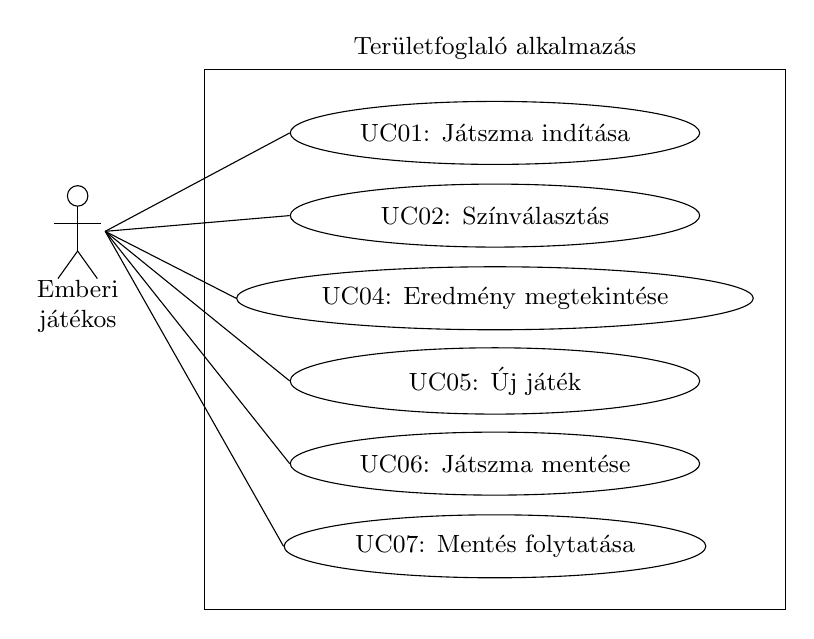
\begin{tikzpicture}[font=\small,
  eset/.style={ellipse,draw,align=center,minimum width=52mm,
    minimum height=8mm}]
\node[eset] (start) at (3.5,0) {UC01: Játszma indítása};
\node[eset] (move) at (3.5,-1.05) {UC02: Színválasztás};
\node[eset] (result) at (3.5,-2.1) {UC04: Eredmény megtekintése};
\node[eset] (restart) at (3.5,-3.15) {UC05: Új játék};
\node[eset] (save) at (3.5,-4.2) {UC06: Játszma mentése};
\node[eset] (resume) at (3.5,-5.25) {UC07: Mentés folytatása};
\node[draw,fit=(start)(move)(result)(restart)(save)(resume),inner sep=4mm,
  label=above:{Területfoglaló alkalmazás}] {};
\draw (-1.8,-0.8) circle (0.13);
\draw (-1.8,-0.93)--(-1.8,-1.5);
\draw (-2.1,-1.15)--(-1.5,-1.15);
\draw (-1.8,-1.5)--(-2.05,-1.85);
\draw (-1.8,-1.5)--(-1.55,-1.85);
\node[align=center] at (-1.8,-2.2) {Emberi\\játékos};
\foreach \cel in {start,move,result,restart,save,resume}
  \draw (-1.45,-1.25)--(\cel.west);
\end{tikzpicture}
\end{center}

\textbf{UC01 -- Játszma indítása (F01).}

\textbf{Aktor:} emberi játékos. \textbf{Előfeltétel:} a beállítási nézet nyitva van.
\textbf{Kiváltó esemény:} az ,,Indítás'' gomb megnyomása.
\begin{enumerate}
\item A játékos megadja a résztvevők számát és típusát.
\item A rendszer ellenőrzi a beállítást, elkészíti a pályát és az induló területeket.
\item Megjelenik a kezdő állás; a kezdő ember színt választhat,
  gépi kezdő esetén az UC03 indul.
\end{enumerate}
\textbf{Eltérés:} érvénytelen beállításnál hibaüzenet jelenik meg,
  a beállítás javítható, játszma nem indul.
\par\textbf{Utófeltétel:} érvényes játszma jött létre, vagy a beállítások változatlanok.

\textbf{UC02 -- Emberi lépés (F02--F03, F05).}

\textbf{Aktor:} az aktuális emberi játékos.
\textbf{Előfeltétel:} futó játszma, emberi kör.
\textbf{Kiváltó esemény:} egy színgomb aktiválása.
\begin{enumerate}
\item A rendszer ellenőrzi a választás szabályosságát és az aktuális kört.
\item Átszínezi a teljes területet, végrehajtja a láncfoglalást,
  és frissíti a pontszámokat és a semleges mezők számát.
\item Ha maradt semleges mező, a következő játékos kapja a kört;
  különben az UC04 következik.
\end{enumerate}
\textbf{Eltérés:} tiltott vagy ismételt választás nem változtatja meg az állást.
  Nulla növekedésű, szabályos lépésnél is továbbadódik a kör.
\par\textbf{Utófeltétel:} pontosan egy teljes lépés történt, vagy a korábbi állapot maradt meg.

\textbf{UC03 -- Gépi kör (F04).}

\textbf{Résztvevő:} belső gépi játékos.
\textbf{Előfeltétel:} futó játszma, gépi kör.
\textbf{Kiváltó esemény:} a vezérlés gépi résztvevőre vált.
\begin{enumerate}
\item A rendszer kijelzi az aktuális gépet, és nem enged emberi lépést.
\item A gép megvizsgálja a szabályos színek teljes foglalási nyereségét,
  majd a mohó szabály szerint választ.
\item A közös szabálykezelő végrehajtja a lépést; a következő kör
  vagy az UC04 következik.
\end{enumerate}
\textbf{Eltérés:} nulla nyereségnél is szabályos színválasztás történik.
  Megszakított játszmába a gépi eredmény már nem kerülhet vissza.
\par\textbf{Utófeltétel:} egy gépi lépés végrehajtódott, vagy a megszakított játék megmarad lezártnak.

\textbf{UC04 -- Eredmény megtekintése (F06).}

\textbf{Aktor:} emberi játékos.
\textbf{Előfeltétel:} a pályán nem maradt semleges mező.
\textbf{Kiváltó esemény:} a rendszer felismeri a befejezési feltételt.
\begin{enumerate}
\item A rendszer lezárja a játszmát, és letiltja a további lépéseket.
\item Megjeleníti a végső pályát, a pontszámokat és a győztest.
\item A játékos megtekinti az eredményt, majd új játékot kezdeményezhet.
\end{enumerate}
\textbf{Eltérés:} azonos legnagyobb pontszámnál döntetlen jelenik meg
  az érintett játékosokkal. A befejezést induláskor is ellenőrizni kell.
\par\textbf{Utófeltétel:} a változatlan végső állapot és eredmény látható.

\textbf{UC05 -- Új játék kezdeményezése (F06).}

\textbf{Aktor:} emberi játékos.
\textbf{Előfeltétel:} játék- vagy eredménynézet látható.
\textbf{Kiváltó esemény:} az ,,Új játék'' gomb megnyomása.
\begin{enumerate}
\item A rendszer megszünteti a korábbi játszmát és annak függő gépi műveleteit.
\item Megnyitja a beállítási nézetet.
\item Új indításkor az UC01 új véletlen pályát készít.
\end{enumerate}
\textbf{Eltérés:} félbehagyott játszmához a rendszer nem hirdet eredményt.
\par\textbf{Utófeltétel:} nincs aktív korábbi játszma; új játék állítható be.

\textbf{UC06 -- Játszma mentése (F07).}

\textbf{Aktor:} emberi játékos.
\textbf{Előfeltétel:} futó játszma, emberi kör, nincs feldolgozás alatt lépés.
\textbf{Kiváltó esemény:} a ,,Mentés'' gomb megnyomása.
\begin{enumerate}
\item A rendszer pillanatképet készít a teljes, érvényes játszmaállapotról.
\item Eltárolja a helyi mentési helyen, a korábbi mentés helyére.
\item Sikeres mentést jelez; a folyamatban lévő játék folytatható.
\end{enumerate}
\textbf{Eltérés:} nem elérhető vagy megtelt tárolónál hibát jelez,
  a futó játék változatlan marad. A művelet nem hajt végre játékbeli lépést.
\par\textbf{Utófeltétel:} siker esetén ugyanaz az állapot később visszatölthető;
  hiba esetén nem jelenik meg sikeres mentésről szóló visszajelzés.

\textbf{UC07 -- Mentett játszma folytatása (F08).}

\textbf{Aktor:} emberi játékos.
\textbf{Előfeltétel:} a beállítási nézet nyitva van, nincs aktív játszma.
\textbf{Kiváltó esemény:} a ,,Folytatás'' gomb megnyomása.
\begin{enumerate}
\item A rendszer beolvassa a helyi mentést, és ellenőrzi annak verzióját és tartalmát.
\item Visszaállítja a pályát, a résztvevőket és az aktuális kört;
  a pontszámokat az eltárolt tulajdonosokból állítja elő.
\item Megjeleníti a mentett állást; a mentéskor soron következő ember léphet.
\end{enumerate}
\textbf{Eltérés:} hiányzó, sérült vagy érvénytelen mentésnél hibaüzenet jelenik meg,
  részleges játékállapot nem jön létre. A felhasználó indíthat új játszmát.
\par\textbf{Utófeltétel:} a mentett játék azonos állapotból folytatódik,
  vagy a rendszer a beállítási nézetben marad.

\section{Fogalomtár}
\begin{tabularx}{\linewidth}{@{}lY@{}}
\toprule
Fogalom & Jelentés \\
\midrule
Szomszéd & Közös éllel rendelkező mező; a csúcsérintés nem számít. \\
Semleges mező & Tulajdonos nélküli, még elfoglalható mező. \\
Terület & Egy játékos összefüggő, egyszínű mezőhalmaza. \\
Lépés & Egy színválasztás és az abból következő teljes foglalás. \\
Pontszám & A játékos területének mezőszáma. \\
Mentés & A folytatáshoz szükséges teljes játszmaállapot tartós pillanatképe. \\
\bottomrule
\end{tabularx}

\section{Technikai paraméterek és tervezett architektúra}
Az alkalmazás \textbf{C\# nyelven, .NET 10 platformon, önálló Blazor
WebAssembly alkalmazásként} készül. A játéklogika a böngészőben fut;
a publikált alkalmazást statikus HTTP(S)-kiszolgáló szolgálja ki.
A felhasználónak nem szükséges .NET-et telepítenie. Célkörnyezet az
aktuális stabil Chrome és Edge asztali böngésző, legalább
1280~$\times$~720-as ablakmérettel. A hexpálya SVG-elemekből rajzolható.

A rendszer áttekintése:
\begin{center}
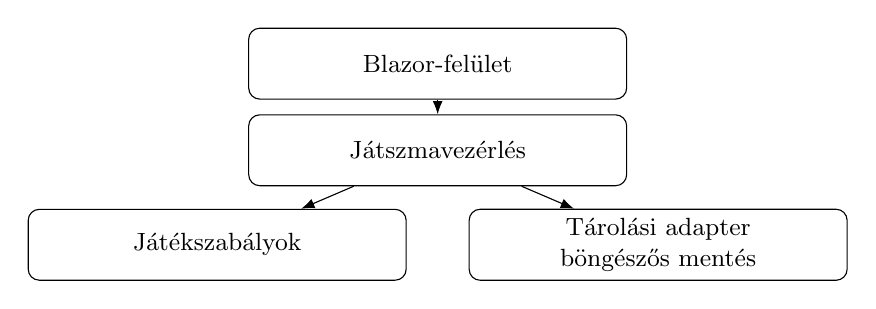
\begin{tikzpicture}[font=\small,
  modul/.style={draw,rounded corners,align=center,minimum width=48mm,
    minimum height=9mm}, nyil/.style={-{Latex}}]
\node[modul] (ui) at (0,1.1) {Blazor-felület};
\node[modul] (app) at (0,0) {Játszmavezérlés};
\node[modul] (rules) at (-2.8,-1.2) {Játékszabályok};
\node[modul] (store) at (2.8,-1.2) {Tárolási adapter\\böngészős mentés};
\draw[nyil] (ui)--(app);
\draw[nyil] (app)--(rules);
\draw[nyil] (app)--(store);
\end{tikzpicture}
\end{center}
A három alapréteget külön adatelérési adapter egészíti ki:

\begin{tabularx}{\linewidth}{@{}lY@{}}
\toprule
Réteg & Felelősség \\
\midrule
Megjelenítés & Beállítások, pályarajzolás, színválasztás, állás és eredmény. \\
Alkalmazásvezérlés & Játszma indítása, körök és gépi lépések vezérlése,
új játék, mentés és folytatás kezelése. \\
Játékszabályok & Hexszomszédság, szabályos színek, foglalás, pontozás
és befejezés. A felülettől függetlenül tesztelhető. \\
Adatelérés & Játszmapillanatkép szerializálása, helyi tárolása és beolvasása. \\
\bottomrule
\end{tabularx}

A megjelenítés a játszmavezérlőn keresztül kér műveleteket
(\textbf{Facade} minta). A gép és az ember ugyanazt a szabálykezelőt
használja. A modell külön tárolja a mező színét és tulajdonosát.
A foglalás a hexszomszédsági gráf bejárásával valósítható meg.

Az aktív állapotot a játszmavezérlő őrzi. A tárolási adapter az
alkalmazásréteg által meghatározott interfészt valósítja meg;
a játékszabályok nem függenek a böngészős tárolástól.
A részletes osztály- és
algoritmusterv, valamint a telepítési leírás külön dokumentációban készül.

\subsection*{Perzisztencia}
A mentés verziózott JSON-pillanatkép a böngésző \texttt{localStorage}
tárolójában. Tartalmazza a mezők színét és tulajdonosát, a résztvevők
típusát, kezdőmezőjét és színét, a sorrendet és az aktuális játékost.
Az adapter a böngésző tárolóját Blazor JavaScript-interoperabilitással éri el.

Visszatöltéskor az alkalmazás ellenőrzi a mezőszámot, az azonosítókat,
a színeket és a játszma konzisztenciáját, mielőtt az állapotot elfogadná.
A mentés ugyanazon webcímen, ugyanabban a böngészőprofilban érhető el.
Oldalújratöltéskor a nem mentett változások elvesznek; a mentett állás
a ,,Folytatás'' művelettel visszaállítható. Böngészőadatok törlése a mentést
is törli. Nincs szükség központi adatbázisra vagy játékot vezérlő szerverre.

\section{Követelmények}
\textbf{M01 -- Helyesség.}
Egy mezőnek legfeljebb egy tulajdonosa van; a terület összefüggő,
egyszínű és tartalmazza a kezdőmezőt. A pontszámok és a semleges mezők
számának összege 120. Ismételt vagy elavult művelet nem okozhat újabb lépést.

\textbf{M02 -- Használhatóság.}
Magyar feliratok és áttekinthető pálya, játékoslista és színválasztó.
Az aktuális játékos egyértelmű. A tulajdonost játékosszám is jelzi,
a színgombokhoz szöveges színnév tartozik.

\textbf{M03 -- Válaszidő.}
A betöltött alkalmazásban az emberi és gépi lépés eredménye egy
másodpercen belül megjelenik a 120 mezős pályán. Ellenőrzése a bemutató
laptopon, Release builddel történik; a gép adatai a tesztjegyzőkönyvbe kerülnek.

\textbf{M04 -- Karbantarthatóság.}
A három réteg felelőssége és függősége elkülönül. A színválasztás,
láncfoglalás, körváltás és eredmény automatizált .NET-tesztekkel,
böngésző nélkül ellenőrizhető.

\textbf{M05 -- Bemenetkezelés és biztonság.}
A beállítások és a lépések érvényességét a logika is ellenőrzi.
Nyilvános webes kiszolgálás HTTPS-en történik. Fiók és adatgyűjtés nincs;
a rendszer helyi, megbízható résztvevők közös játékára készül.

\textbf{M06 -- Tartós állapot helyessége.}
Mentés és böngésző-újraindítás utáni folytatáskor a pálya, a résztvevők
és az aktuális kör egyeznek. Hibás mentés nem indíthat érvénytelen játszmát;
tárolási hiba nem módosíthatja a futó állapotot.

\end{document}
